% !TEX TS-program = pdflatex
% !TEX encoding = UTF-8 Unicode

\documentclass[11pt]{report} % use larger type; default would be 10pt

\usepackage[utf8]{inputenc} % set input encoding (not needed with XeLaTeX)

\usepackage{listings} % source code formatting
\usepackage{hyperref}
%%% Examples of Article customizations
% These packages are optional, depending whether you want the features they provide.
% See the LaTeX Companion or other references for full information.

%%% PAGE DIMENSIONS
%\usepackage{geometry} % to change the page dimensions
%\geometry{a4paper} % or letterpaper (US) or a5paper or....
% \geometry{margin=2in} % for example, change the margins to 2 inches all round
% \geometry{landscape} % set up the page for landscape
%   read geometry.pdf for detailed page layout information

\usepackage{graphicx} % support the \includegraphics command and options

% \usepackage[parfill]{parskip} % Activate to begin paragraphs with an empty line rather than an indent

%%% PACKAGES
\usepackage{booktabs} % for much better looking tables
%\usepackage{array} % for better arrays (eg matrices) in maths
\usepackage{paralist} % very flexible & customisable lists (eg. itemize/itemize, etc.)
\usepackage{verbatim} % adds environment for commenting out blocks of text & for better verbatim
\usepackage{subfig} % make it possible to include more than one captioned figure/table in a single float
% These packages are all incorporated in the memoir class to one degree or another...

%%% HEADERS & FOOTERS
\usepackage{fancyhdr} % This should be set AFTER setting up the page geometry
\pagestyle{fancy} % options: empty , plain , fancy
\renewcommand{\headrulewidth}{0pt} % customise the layout...
\lhead{Smart Water Network Monitor}\chead{}\rhead{}
\lfoot{}\cfoot{\thepage}\rfoot{}

\usepackage{usecases}

%%% SECTION TITLE APPEARANCE
\usepackage{sectsty}
\allsectionsfont{\sffamily\mdseries\upshape} % (See the fntguide.pdf for font help)
% (This matches ConTeXt defaults)

%%% ToC (table of contents) APPEARANCE
\usepackage[nottoc,notlof,notlot]{tocbibind} % Put the bibliography in the ToC
\usepackage[titles,subfigure]{tocloft} % Alter the style of the Table of Contents
\renewcommand{\cftsecfont}{\rmfamily\mdseries\upshape}
\renewcommand{\cftsecpagefont}{\rmfamily\mdseries\upshape} % No bold!
\renewcommand{\chaptername}{}

\usepackage{titlesec}
\usepackage{lipsum}
\titleformat{\chapter}
{\filcenter\normalfont\LARGE\bfseries}
{\chaptertitlename~\thechapter} {0.5em} {}


%%% END Article customizations

%%% The "real" document content comes below...

\title{Smart Water Networks Monitor}
\author{Abhijith Madhav, Kumudini Kakwani}
%\date{} % Activate to display a given date or no date (if empty),
         % otherwise the current date is printed 

\begin{document}
\maketitle

\tableofcontents

\chapter{Introduction}
\section{Problem}
Water needed for the IIIT-B campus is sourced in three ways
\begin{enumerate}
\item
IIITB has its own source of water in the form of three functional borewells. Water is pumped out of these borewells for almost twenty hours a day. 
\item
Water supply from BWSSB for a limited amount of time each day.
\item
Almost 20000-30000 liters of water per day is procurred from commercial water tankers.
\end{enumerate}
Currently there is no insight into how water is being used and about whether its use is optimal or not. Informal estimates term the per-capita water consumption within the campus as excessive.

\section{Objective}
There is a proposal to make the water distribution network of the IIIT-B campus a smart one with the installation of sensors in the network. Our system intends to plug into this smart network and work on the data that the sensors produce. \\

Specifically this project intends to
\begin{enumerate}
\item
Be general purpose enough to plug into any small to medium sized smart water network(An institute, a corporate campus, a gated community, a farm etc)
\item
Help in better water management by offering insights into water usage across the network.
\item
Help in maintaining the water network by detection and reporting of anomalous events.
\end{enumerate}

\section{External Dependencies and Assumptions}
\begin{enumerate}
\item
Installation of flow, quality and level sensors at suitable points in the water network to make it a smart one. 
\item
Installation of a SCADA like system with a ODMS(A historian) from where sensor data can be read off.
\end{enumerate}
In the absence of the above we have implemented a stop-gap sensors simulator which will fill database with psuedo sensor data until real sensors are deployed in the network.

%-----------------------------------------------------------------

\chapter{Scope And Requirements}

The focus was on architecting, designing and implementing the below
\begin{enumerate}
\item
Supervisor mobile apps which
\begin{itemize}
\item
Detail water usage patterns.
\item
Notify user on anomalous events and other happenings in the water network.
\end{itemize}
\item
Architecting and implementing a modular backend storage system to
\begin{itemize}
\item
Represent the smart water network.
\item
Manage all the data generated by the sensors.\\
\end{itemize}
\end{enumerate}
We are limiting the extent of our implementation to \textbf{not} include the below
\begin{enumerate}
\label{itm:todo}
\item
The mobile app for field personnal which assigns issues to them and helps them update the status of these issues.
\item
Web UI's to construct the smart water network. We will load the structure of the smart water network in batch mode to our backend systems and then work on the same.
\item
A visual geospatial representation of the water network where a centralized view of the whole network is possible. Here each network asset has a visual representation and its parameters can be inspected by clicking on them.
\end{enumerate}
\section{Use Cases}
\begin{usecase}
\addtitle{Use Case 1}{Insights into the water network}
\addfield{Actors}{Administrators}
\additemizedfield{Activities}{
\item Will be able to see the breakdown of water usage across aggregations with options to drill down to specific granularity. Aggregations can be buildings, blocks, floors etc. Aggregations can be nested.
\item Will be able to inspect health parameters of the water network. Health parameters can quality of water, electricity used, level of water in storage etc.
}
\end{usecase}

\begin{usecase}
\addtitle{Use Case 2}{Predictions}
\addfield{Actors}{Administrators}
\additemizedfield{Activities}{
\item Will get predictions regarding future water usage based on historical water usage patterns so that planning for rationing/procurement of water can be done.
}
\end{usecase}

% ----------------------------------------------------------------------------------

\chapter{Architecture And Design}

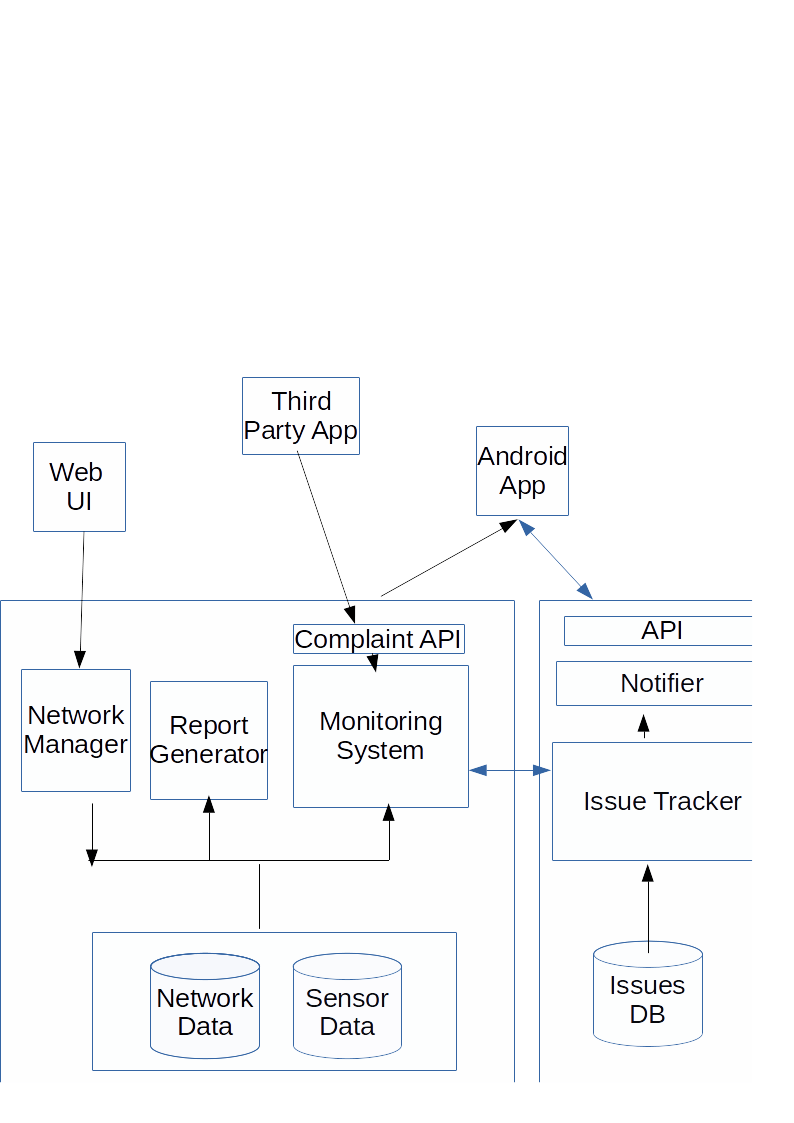
\includegraphics[scale=0.4]{HLD.png}

\section{Application Backend}
\subsection{Data Store Design}
\subsubsection{Representing The Water Network}
The water network representation is stored in a relational database(mysql). The schema for the same is documented below. Common properties across all assets are stored in the asset table whereas differing properties are stored in an EAV table. A EAV based table is being used to enable future addition of different assets with different properties into the database without change of schema of the database or proliferation of tables.

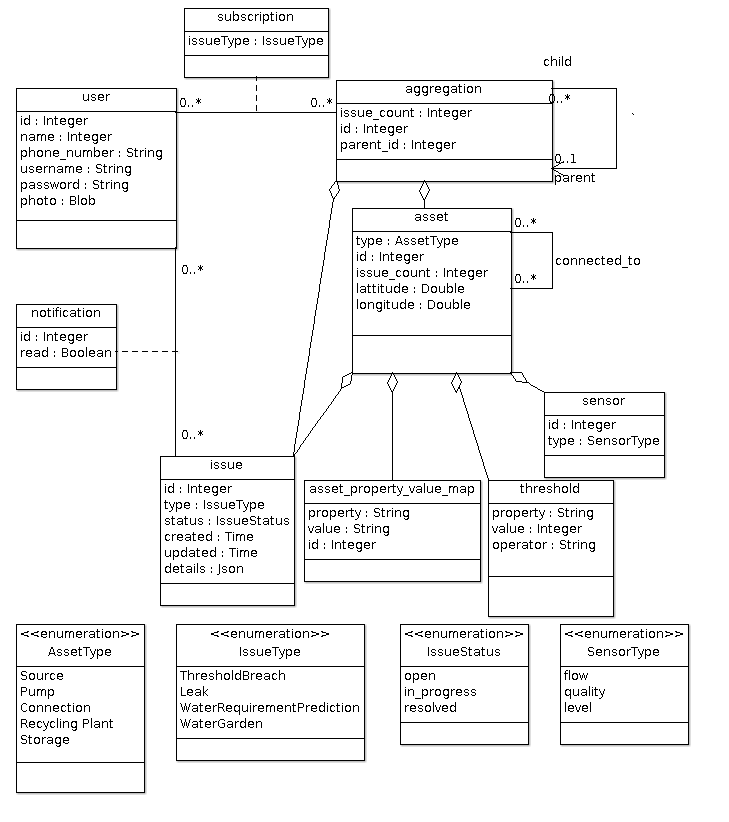
\includegraphics[scale=0.4]{DBDesign.png}
\subsubsection{Storing Sensor Data}
The sensor(psuedo) data is stored in a time series database(Influxdb) to help with time based queries. The entry point for this data is the sensor id which is stored in the network database.
\begin{itemize}
\item The sensor id represented in the assets table is an application defined reference to entries in a time series database table.
\item All sensors(data simulator) write to a table(sensors) in the time series database,  entries of which have the following structure.
\begin{lstlisting}
{
      sensor_id : <sensor id>,
      label1 : <value for label1>,
      label2 : <value for label2>,
      .
      .
      .
}
\end{lstlisting}
\end{itemize}
\subsection{Monitoring System}
Scans the sensor data continuously for anomalies and reports the same to the issue tracker. Anomalies include breaches in threshold levels, leaks(not implemented) and external complaints(not implemented). It also reports daily water requirements according to it's prediction(Not implemented).
\subsubsection{Data Simulator}
This module simulates the sensors in the network and generates psuedo sensor data.
\subsection{Web Application}
\label{sec:web_application_api}
Provides an REST API to query  the following entities
\begin{itemize}
\item Notifications.
\item Aggregations
\item Assets
\end{itemize}
Provides a non-REST API to get the below data
\begin{itemize}
\item Water consumption break up.
\item Water consumption by time.
\end{itemize}
\section{Android Application}
The android application provides 3 main view.
\subsection{Notifications}
Shows notifications by consuming the Notifications REST API provided by the backend
\subsection{Reports}
Generates two reports, one on the water consumption break up and the other on the water consumption trend. Consumes the Non-REST API provided by the backend for the same.
\subsection{Network Health}
Provides a hierarchical view of the health of the network.

%-----------------------------------------------------------------------------

\chapter{Technology And Implementation}
The entire source code is versioned at \url {https://github.com/smartwatermanagement/self-healing-water-networks}.

\section{Data Store}
The relational database used is MySQL. A database dump is available at \texttt{/SWNBackend/DB SQL FIle/swndb.sql}
The DAO's for access of the same are at \texttt{/SWNBackend/src/dao}
The current database contains a sample water network shown below.
%TODO : Add picture

Sensor data is stored in a time series database called InfluxDB. When the actual sensors are deployed it is hoped that only a sensors data access object will have to be implemented. The current DAO object is at \texttt{/SensorsDataDAO}

\section{Monitoring System}
\texttt{/MonitoringSystem}\\
\\
A multi-threaded application which spawns of threads to do the following
\begin{itemize}
\item Generate pseudo data for the sensors table.
\item Detect breaches in threshold levels set for sensors.
\item Leak detector(Dummied for now).
\item Water requirement predictor(Dummied for now).
\end{itemize}


\section{Web Application}
\texttt{/SWNBackend} \\
\\
The web application is hosted inside an Apache J2EE application container. It uses the \textbf{ Struts2} framework to establish an MVC architecture. Further the \textbf{Struts2 REST plugin} and the \textbf{Struts2 JSON plugin} are used to set up REST API's.
\\
\noindent

\subsection{Constructing The Water Network}
\texttt{/SWNBackend/src/model/WaterNetwork.java}
\\
\noindent The structure of the network is read from the database only once, when it is referred to for the first time, after the application backend is bought up. It is expected that updates to the network when implemented in future write through the memory.
\noindent The representation of the network looks like a forest of trees each rooted at a source or a storage asset node after construction.

\subsection{Calculating Water Usage And Trends}
\texttt{/SWNBackend/src/action/nonrest}
\\
\noindent The above required data are calculated by traversing up and down the water network data structure and getting the requisite flow data by making calls to the sensor database.

\chapter{Status Of Completion}
\section{Completed}
\begin{itemize}
\item Android application for the supervisor.
\item Application backend which supports the API's listed in ~\ref{sec:web_application_api}
\end{itemize}
\section{To Do}
\begin{itemize}
\item Algorithms for detecting leaks and predicting water requirements.
\end{itemize}


\chapter{Test Summary}
\chapter{Open Issues}
\begin{itemize}
\item JSON error reponses
\item Implement a color picker for the 
\end{itemize}
\chapter{Suggested Enhancements}
\begin{itemize}
\item Push notifications in the android applications using Google Cloud Messaging infrastructure.
\item When there are multiple notifications for the same asset, collapse them.
\item Leak detection algorithm.
\item Water prediction algorithm.
\item The location information in the asset view and in the details of a notification must open out into a terrain map which shows the route from the current location to the asset location instead of displaying latitude and longitude
\item Features listed in ~\ref{itm:todo}
\end{itemize}
\chapter{Installation Notes}
\begin{itemize}
\item Clone repository \url {https://github.com/smartwatermanagement/self-healing-water-networks}
\item Install MySQL
\item Create a database and create schema using dump file  \texttt{/SWNBackend/DB SQL FIle/swndb.sql}
\item Install influxDB
\item Run the monitoring system, \texttt{/MonitoringSystem}
\item Run \textbf{Apache} with the WAR of the application deployed.
\item Install the android app 
\end{itemize}
\end{document}
